\chapter{Introduction} \label{introduction}

\gls{dna} sequencing allows us to read an organism's genome and, through 
software, learn more about organism's inherent capabilities without having to 
study it \textit{in vivo} or \textit{in vitro} \cite{de2012bioinformatic}. In an 
environmental microbiology context, such sequenced genomes are used to learn 
more about microorganisms' metabolic capabilities and possibly shed light on 
their ecological roles \cite{de2012bioinformatic}. In an applied context, 
predictions of such metabolic capabilities are also useful for the selection of 
what microbes to use in a bioprocess. In a genetic engineering context, 
genomically derived information can be used to select what metabolic traits to 
remove from, or move between, organisms 
\cite{strohl2001biochemical,sanchez2005novel}.

Advances in \gls{dna} sequencing technology over the past decade have 
revolutionized our ability to acquire bacterial and archaeal genomes. For 
example, with newer sequencing technologies, such as Oxford Nanopore 
\cite{jain2016oxford}, a bacterial genome can be acquired in a matter of hours 
\cite{Lu2016,Cao2017}. Researchers have now moved on to extracting the genomes 
of unculturable microorganisms from environmental samples using culture-free 
techniques, such as metagenomic \cite{quince2017shotgun} and single-cell 
\cite{gawad2016single} sequencing. Over the past few years, the tree of life has 
been significantly expanded by the \gls{mags} \cite{bowers2017minimum} of these 
unculturable organisms \cite{Hug2016,Parks2017}. With microbiologists' inability 
to gather new genomes rectified, the problem now shifts to interpreting the 
resulting new wealth of genomic data.

Due to their vast size and information density, the interpretation of genomes is 
often assisted by software. The tool that was developed as part of the thesis 
work, Micromeda, allows users to generate data visualizations that help them 
identify patterns in the presence and absence of biochemical pathways across 
organisms. Pygenprop, a library built to assist in the development of Micromeda, 
enables users to perform such comparisons programmatically. A key feature of 
both Micromeda and Pygenprop is their ability to not only compare the predicted 
metabolic features of organisms, in terms of biochemical pathways present, but 
also allow users to access the underlying protein sequences that support these 
predictions. Details about the information presented by Micromeda and its 
expected use cases are presented within the sections below. The following 
chapters will discuss the database Micromeda uses, Pygenprop, and Micromeda's 
implementation.

\section{Enzymes and Biochemical Pathways} \label{enzymes-and-pathways} 

For many systems, both environmental and industrial processes can be carried out 
biochemically. From a biological context, such processes are carried out via a 
series of chemical reactions catalyzed by proteinaceous biological enzymes. 
Enzymes that facilitate similar chemical reactions often have similar sequences 
of amino acid residues, structures, and genes that encode them 
\cite{galperin1998analogous,zhang2003evolution}. 

A protein domain is a conserved subset of a protein's sequence that carries out 
a specific function and is evolutionarily conserved \cite{ren2008conservation}. 
These domains are associated with distinct sequence motifs, which are patterns 
in the protein's amino acid sequence \cite{ren2008conservation}. All enzymes 
have an active site 
(\href{http://en.wikipedia.org/wiki/Active_site}{en.wikipedia.org/wiki/Active\_site}), 
and this active site often has a unique sequence motif. This motif can be used 
to identify specific enzymes or enzyme families uniquely 
\cite{ren2008conservation}. 

A biochemical pathway represents a series of chemical reactions, that when 
chained together, are beneficial to a cell \cite{michal2012biochemical}. 
Examples of such reactions are the breaking down of a nutrient macromolecule 
into pieces that cells can use or the synthesis of components of cellular 
structure \cite{wagner2012metabolic}. Each reaction step in a pathway is often 
\cite{keller2015widespread,tawfik2010enzyme} catalyzed by a specific enzyme 
whose amino acid sequence, and thus structure and activity, is optimized for the 
reaction \cite{michal2012biochemical,zhang2003evolution,fersht1999structure}. 
Thus, there is a mapping between specific enzymes (and the genes encoding them) 
and chemical reaction steps in biochemical pathways \cite{thiele2010protocol}. 
As a result, by reading the genome, researchers can predict what biochemical 
pathways an organism may possess 
\cite{abubucker2012metabolic,thiele2010protocol}. Also, the output from one 
pathway (\textit{e}.\textit{g}., the monomers from the break down of a 
macro-nutrient) may be the input for a second biochemical pathway that builds 
cellular structures \cite{wagner2012metabolic,stelling2002metabolic}. Thus, all 
pathways in a cell are somehow connected and form a network of reactions 
\cite{wagner2012metabolic,stelling2002metabolic}. This network forms the cell's 
metabolism and is called its metabolic network \cite{wagner2012metabolic}.

\section{The State of Pathway Analysis} \label{pathway-databases}

For many decades scientists have been designing and executing studies to figure 
out what individual enzymes do and what substrates they can catalyze. The 
results of such studies are stored in pathway databases. Specifically, what 
genes encode for what enzymes, what enzymes catalyze what reactions, and what 
reactions belong to what biochemical pathways. These databases also map how 
pathways are connected within cells' metabolic networks. Examples of such 
databases include \gls{kegg} \cite{kanehisa2000kegg}, MetaCyc 
\cite{karp2002metacyc}, Genome Properties \cite{richardson2018genome}, SEED 
subsystems \cite{overbeek2005subsystems}, Reactome \cite{croft2013reactome}, and 
many others.

As the breadth and depth of the information within pathway databases increases, 
the information contained within is increasingly being used by automated tools 
that perform pathway analysis. Such tools help make rapid insights into the 
capabilities and roles of organisms in a variety of environments. Often this 
software is released in the form of a toolchain (\textit{i}.\textit{e}., a 
pipeline) where separate bioinformatics software applications are run in series 
to generate a final output. Such pipelines take an organism's \gls{dna} genome 
sequence, perform \textit{in-silico} transcription and translation (Fig. 
\ref{fig:pathway-analysis-steps}), identify enzymes, and identify the pathways 
that these enzymes support via information contained within pathway databases (Fig. 
\ref{fig:pathway-analysis-overview}). These tools perform some or all of the 
following key steps.

\begin{enumerate}
\item Prediction of what genes are present in an organism's genome.
\item Translation of these genes' sequences to protein for reduced redundancy 
(Fig. \ref{fig:pathway-analysis-steps}).
\item Taking known enzymatic protein sequences from pathway databases and using 
these sequences to search the predicted proteins to find those with high 
sequence similarity. Predicted proteins with high sequence similarity to known 
enzymes are likely to carry out the same enzymatic function (see Section 
\ref{enzymes-and-pathways}). This process is called protein annotation (Fig. 
\ref{fig:pathway-analysis-steps}).
\item Using these newly found enzymes to figure out what chemical reactions 
could be carried out by an organism.
\item Chaining these reactions together to figure out what biochemical pathways 
are likely to be possessed by the organism (Fig. 
\ref{fig:pathway-analysis-steps}). This process is called pathway annotation.
\item Presentation of information about the pathways present and enzymes found 
in a way that is comprehensible by users.
\end{enumerate}

\begin{figure}[!ht]
  \centering
	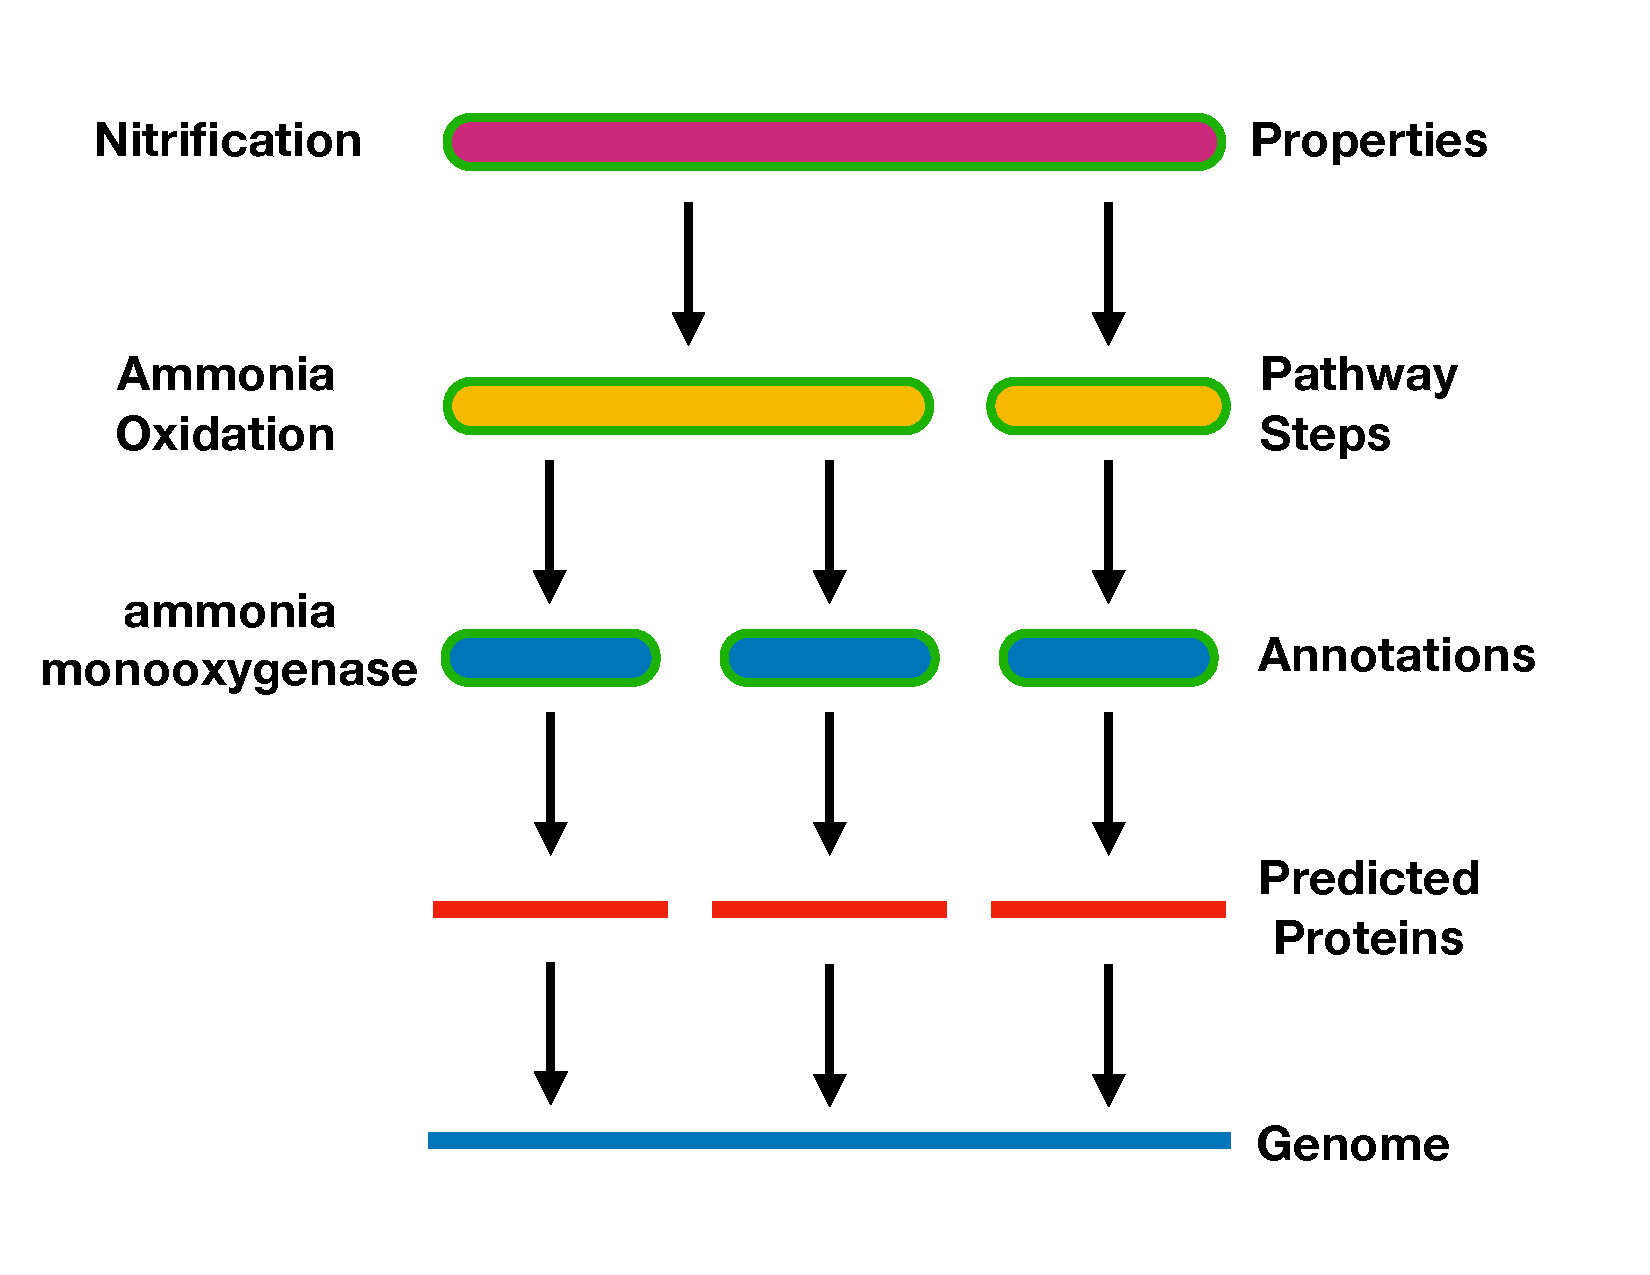
\includegraphics[width=0.9\textwidth]{media/pathway_analysis_steps.pdf}
\caption[How the glyoxylate shunt can be predicted from the presence of its 
supporting enzymes.]{\textbf{How the glyoxylate shunt can be predicted from the 
presence of its supporting enzymes.}  If a microorganism is to be classified as 
possessing a glyoxylate shunt, then it should have highly similar proteins to 
those previously known to carry out the pathway, such as Iso and MalG. Several 
steps are required to go from an organism’s genome sequence to a prediction of 
its metabolic capabilities. The enzymes that carry out the pathway steps must be 
identified (\textit{e}.\textit{g}., protein annotation). If found, these enzymes 
would indicate the presence of pathway steps. Finally, if all or many steps are 
present, then the biochemical pathway can be said to be present.}
	 \label{fig:pathway-analysis-steps}
\end{figure}

\begin{figure}[!ht]
  \centering
	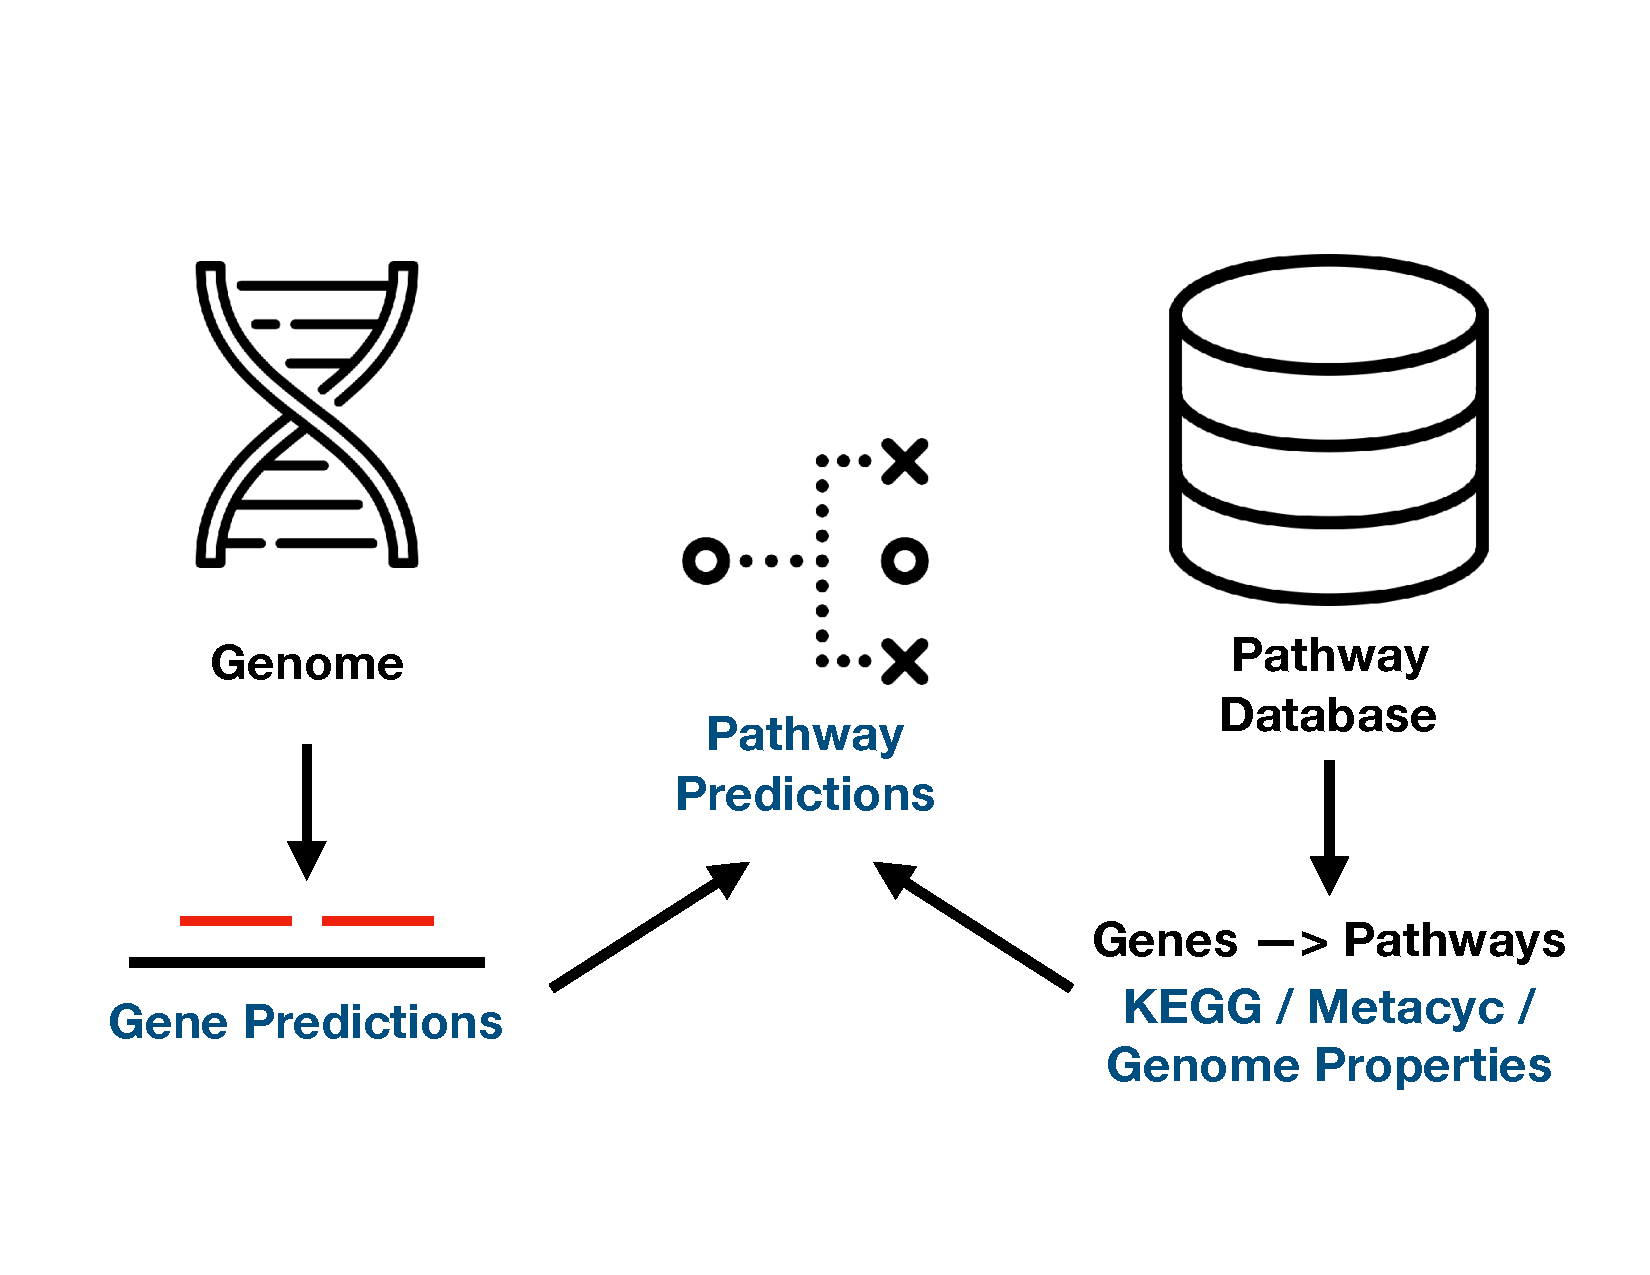
\includegraphics[width=0.8\textwidth]{media/pathway_bioinformatics.pdf}
	\caption[How an organism’s biochemical pathways are genomically predicted using 
information from pathway databases.]{\textbf{How an organism’s biochemical 
pathways are genomically predicted using information from pathway databases.} 
Predicting an organism’s biochemical pathways involves joining together two 
distinct datasets. One is a prediction of what genes are possessed by an 
organism. The other is a database containing the knowledge of what genes are 
involved in previously known biochemical pathways. When predicted proteins with 
sufficient homology to the previously cataloged genes are found within an 
organism’s genome, pathway prediction can be made.}
	 \label{fig:pathway-analysis-overview}
\end{figure}

Users can deploy pathway prediction bioinformatics pipelines in two ways. The 
pipelines can either be installed on to a user's computer, where genomes can be 
processed directly, or be deployed on to a web server, where users can upload 
their genomes for remote processing. Some pipelines only work with pathway data 
from a specific database. For example, Pathway Tools \cite{karp2002pathway} can 
only present information about pathways found within the MetaCyc 
\cite{karp2002metacyc} database. Often pipelines are optimized for generating 
data from the genomes of a specific clade on the tree of life. For example, 
Prokka \cite{seemann2014prokka}, a pipeline that predicts genes and annotates 
protein sequences, is only designed to work with the genomes of prokaryotic 
microbes. Prokka only carries out the first two steps of the key pathway 
analysis steps listed at the top of this section \cite{seemann2014prokka}. Once 
these proteins are predicted, they can be uploaded to servers such as \gls{kaas} 
\cite{moriya2007kaas} for pathway annotation. Several tools can perform all of 
the pathway analysis steps outlined in the key pathway analysis steps list. For 
example, \gls{rast} \cite{aziz2008rast} can take the upload of whole or partial 
bacterial genomes, predict the genes of these genomes, and provide users with a 
report displaying found pathways.

\section{The Current Bottlenecks of High Throughput Pathway Analysis}

Due to the current plethora of tools for genome annotation and pathway 
determination, identifying pathways for single organisms is becoming a solved 
problem. Researchers have progressed to comparing the presence and absence of 
pathways across organisms. Such comparisons are applied in order to, for 
example, find information about individual organism's ecological roles, 
evolution, or suitability towards different industrial tasks. For example, the 
genomes of organisms that are closely related phylogenetically could be compared 
to determine those that may have lost or gained a pathway or pathway step over 
time. Alternatively, the pathways possessed by multiple organisms from within 
the same environment could be compared to shed light on their potential 
ecological niches (Fig. \ref{fig:metagenomics}). Pathway comparisons could also 
be used industrially to select organisms to add to bioprocess co-cultures.

\begin{figure}[!ht]
  \centering
	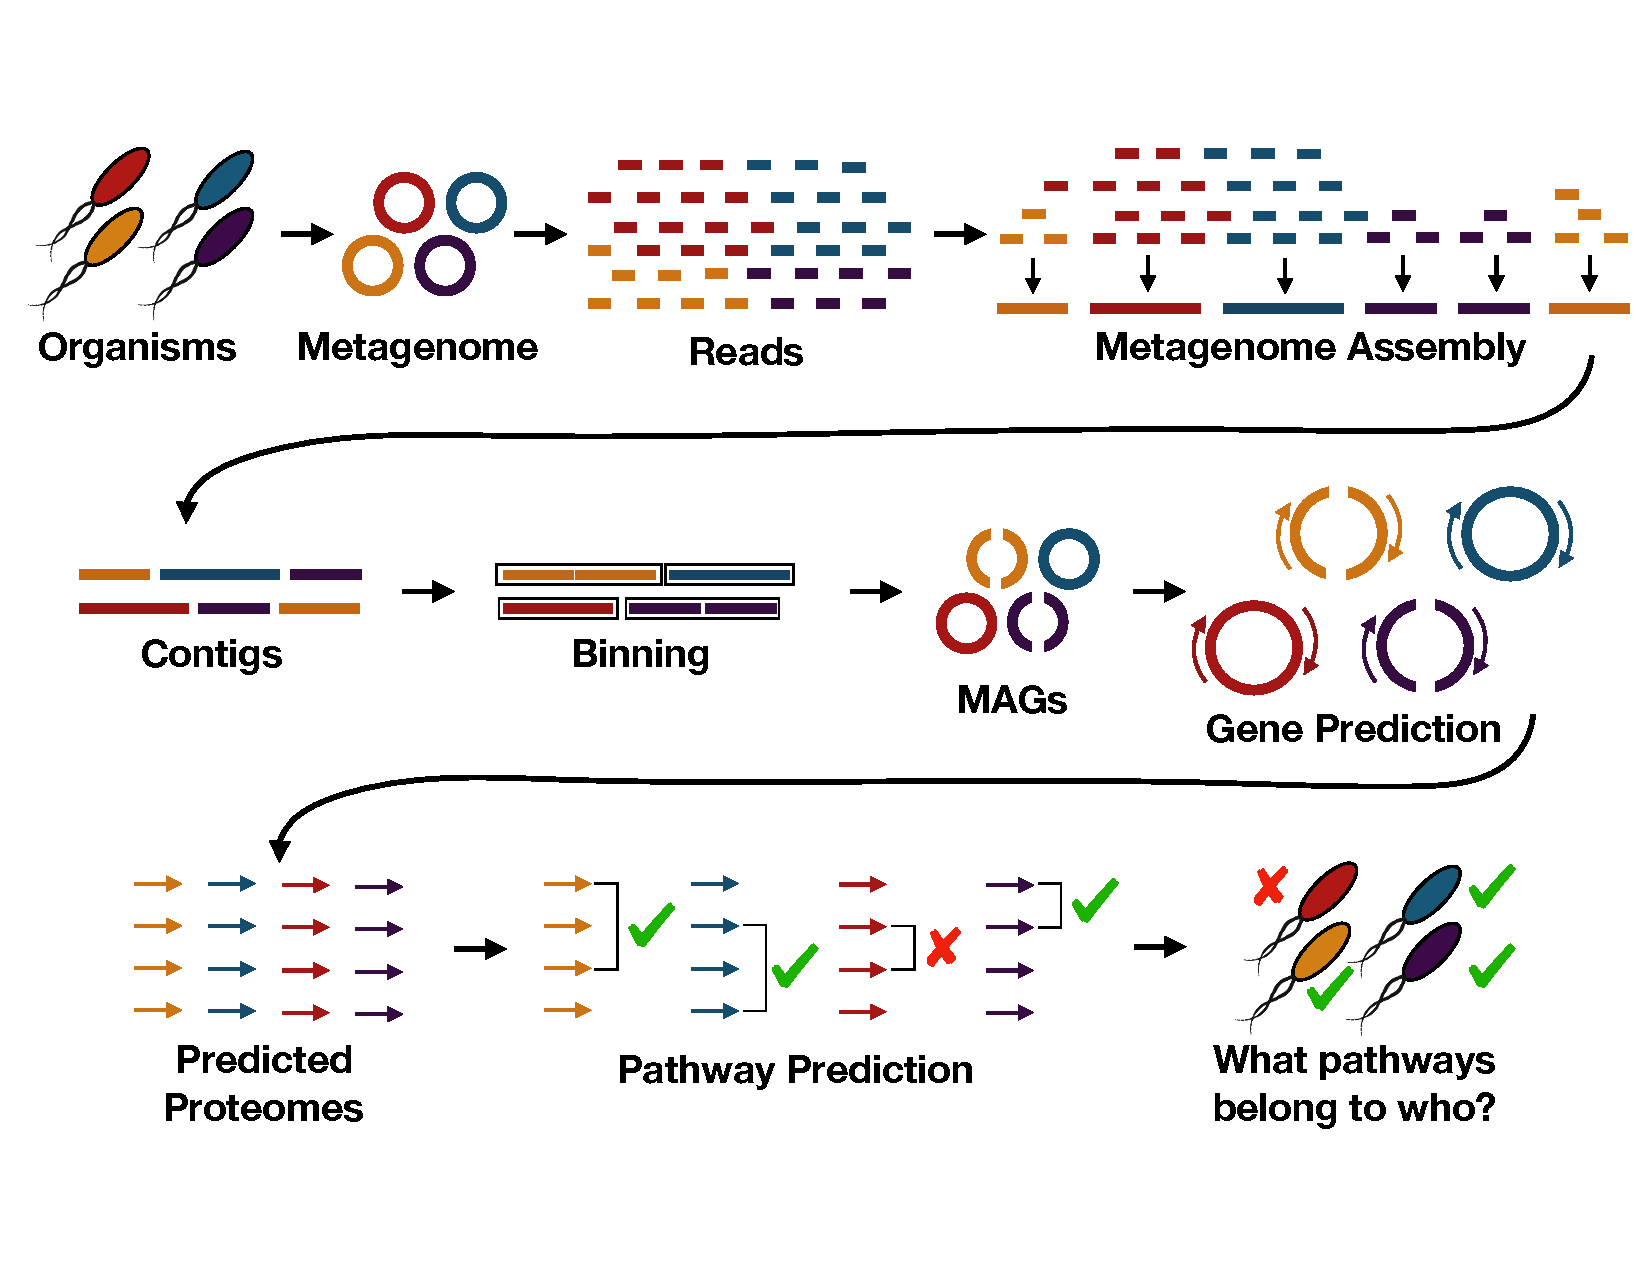
\includegraphics[width=0.75\textwidth]{media/metagenomics.pdf}
	\caption[Metagenomics steps used to determine the biochemical pathways 
possessed by organisms found in a single environment.]{\textbf{Metagenomics 
steps used to determine the biochemical pathways possessed by organisms found in 
a single environment.} Bioinformatics techniques can be used to separate 
individual genomes from a metagenomic sample. Pathway annotation can be 
performed on these genomes and used to compare the pathways possessed by 
different organisms from the same environment. Such comparisons can be used to 
evaluate each organism's potential role in an environment.}
	 \label{fig:metagenomics}
\end{figure}

Although assigning pathway presence and absence to individual organisms can be 
done quite rapidly, the comparison of these results across multiple organisms is 
currently a considerable bottleneck in the area of pathway analysis. Often 
pathway annotation tools that can process multiple genomes simultaneously 
present their results in the form of computer spreadsheets 
(\textit{e}.\textit{g}., Microsoft Excel or \gls{csv} files \cite{RFC4180}). 
After generation of these spreadsheets, users are required to manually scan 
through the thousands of pathway rows and organism columns to find pathway 
differences across organisms. Researchers with data science and coding skills 
may be able to generate custom R or Python scripts that assist them in this task 
by filtering down these spreadsheets to show only pathways that are different or 
by generating data visualizations that accelerate pattern detection. To 
accelerate script development, libraries have been written to help scriptwriters 
interact with pathway data. However, the majority of these libraries focus on 
helping users download data from existing pathway databases, rather than helping 
them with making comparisons across organisms. Thus, due to a lack of libraries 
for pathway comparison and lack of coding skills among biologists, there is a 
need for dedicated bioinformatics tools that simplify pathway comparisons across 
organisms. Software that visualizes the presence and absence of pathways would 
be of great use for performing such comparisons. There are several emerging 
tools, which are discussed in Section \ref{micromeda-client-summary}, that help 
users visualize pathway annotations from multiple organisms. However, these 
software programs' implementation, in terms of visual idioms used and supporting 
data presented, is currently lacking. There is currently a gap for a tool that 
effectively presents such data and allows for rapid comparisons. There is also a 
gap for a pathway library that assists coders in making these comparisons 
programmatically. Finally, there is a gap for a tool that can both describe what 
pathways an organism possesses and allow users to identify the protein sequences 
that support these pathway annotations. Micromeda and Pygenprop were developed 
to fill these gaps.

\section{The Micromeda Platform} \label{micromeda-overview}

The bioinformatics system presented within this thesis, called Micromeda, is 
designed to address current gaps in the researcher's ability to compare pathway 
presence and absence across organisms. The platform generates these comparisons 
without losing information about the protein sequences that support the 
pathways' existence. The output of the platform is an interactive heat map that 
displays rows of pathways by columns of organisms (Fig. 
\ref{fig:basic-heatmap-overview}). Heat map cells are coloured by the level of 
support for a pathway's existence in each genome (Fig. 
\ref{fig:basic-heatmap-overview}). This data visualization is displayed within a 
user's web browser. As discussed in Chapter \ref{micromeda-client}, this heat 
map is interactive, and users can tailor it to only display presence and absence 
for specific pathways or pathway steps. A software stack (see 
\href{http://en.wikipedia.org/wiki/Solution_stack}{en.wikipedia.org/wiki/Solution\_stack}) 
consisting of several components, some of which were developed as part of the 
thesis project, is used to generate data for the visualizations that Micromeda 
presents. This stack is outlined in the list below.

\begin{figure}[!ht]
  \centering
	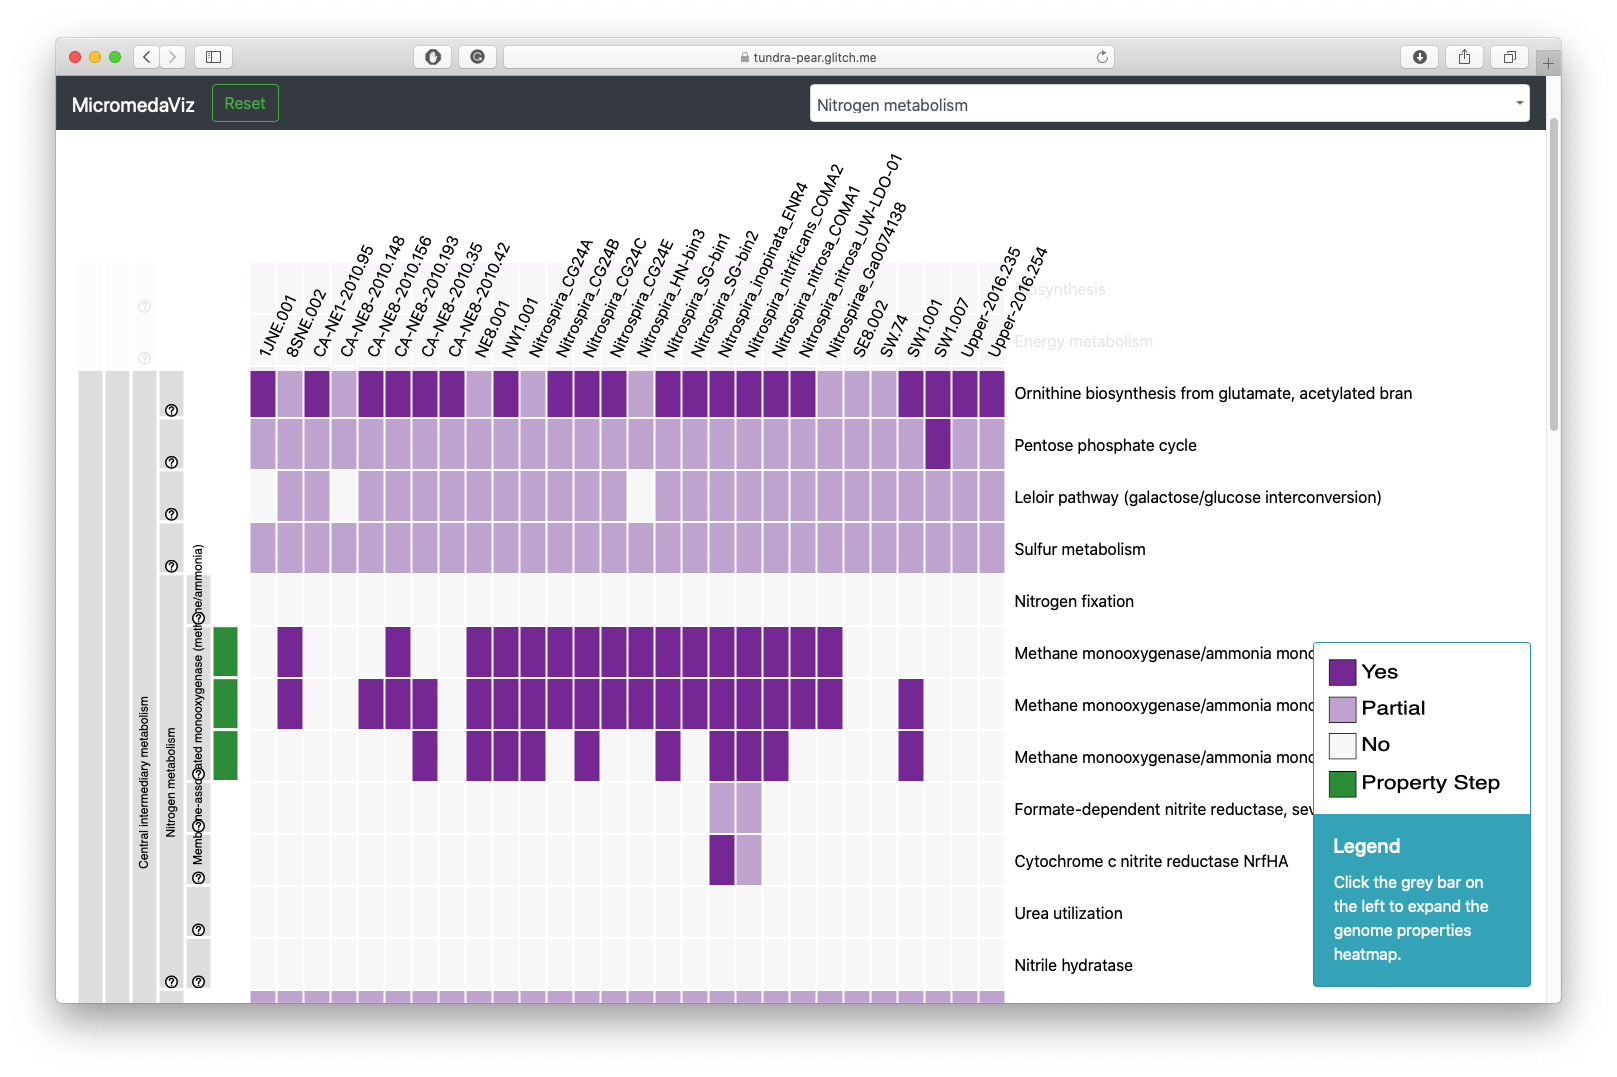
\includegraphics[width=0.9\textwidth]{media/Micromeda-Simple-Overview.png}
	 \caption[Web-browser window containing Micromeda’s heat map visualization 
and interface.] {\textbf{Web-browser window containing Micromeda’s heat map 
visualization and interface.} This heat map consists of pathway rows by organism 
columns and allows the comparison of pathway presence and absence across 
organisms. All other components of Micromeda were built to support this 
interface by providing it with data. Further explanation of the interface’s 
design can be found in Chapter \ref{micromeda-client}.}
	 \label{fig:basic-heatmap-overview}
\end{figure}

\begin{itemize}
\item A program that generates protein sequences from predicted genes found 
within an organism's genome. For example, in the case of prokaryotic genomes, an 
existing tool such as \textbf{Prodigal} \cite{hyatt2010prodigal} would be used. 

\item A pre-existing sequence search program for scanning for identifying 
markers within the sequences of an organism's predicted proteins. These markers 
are used to identify enzymes that support the existence of a pathway. The search 
program chosen was \textbf{InterProScan5}, whose output data are used by the 
Genome Properties Database. An overview of InterProScan5 
\cite{jones2014interproscan} and its methodology can be found in Chapter 
\ref{genome-properties}.

\item A pathway database that maps between predicted protein sequences derived 
from an organism's genome and biochemical pathway steps. The database chosen was 
the \textbf{Genome Properties} database \cite{richardson2018genome}. A short 
review of this database and the reason for its selection can be found in Chapter 
\ref{genome-properties}. This database is pre-existing and was not made as part 
of the thesis work.

\item A software library that supports the generation of pathway annotations, 
rapid programmatic comparisons between organism pathway annotations and the 
generation of Micromeda files. The library is compatible with many 
emerging machine learning tools and opens up new avenues to their application to 
pathway analysis. This library is called \textbf{Pygenprop} and is discussed in 
Chapter \ref{Pygenprop}.

\item A file format that allows users to easily transfer an assessment of what 
pathways are possessed by multiple organisms and the protein sequences used to 
support this assessment. These files, called \textbf{Micromeda files}, are the 
files uploaded to Micromeda-Server and use a custom format that is discussed in 
Section \ref{MicromedaFiles}. The format allows for the storage of the pathway 
and sequence information in the most compact way possible.

\item A server web application that runs on a remote computer system and in 
support of the client application. This server application accepts file uploads 
from the client and provides the client with easy access to the data held within 
the file. This component is called \textbf{Micromeda-Server} and is discussed in 
Chapter \ref{micromeda-server}.

\item A client web application that runs in the user's browser. This web 
application allows users to upload files to a server. These files contain 
precalculated data about an organism's predicted pathways and the protein 
sequences that support these predictions. This application draws pathway 
heat maps based on this uploaded data  (Fig. \ref{fig:basic-heatmap-overview}). 
These heat maps allow users to make comparisons across pathways and organisms. 
This component is called \textbf{Micromeda-Client} and is detailed in Chapter 
\ref{micromeda-client}. Links to a demonstration of the client interface can be 
found in Section \ref{client-demo}.
\end{itemize}

\begin{figure}[!ht]
  \centering
	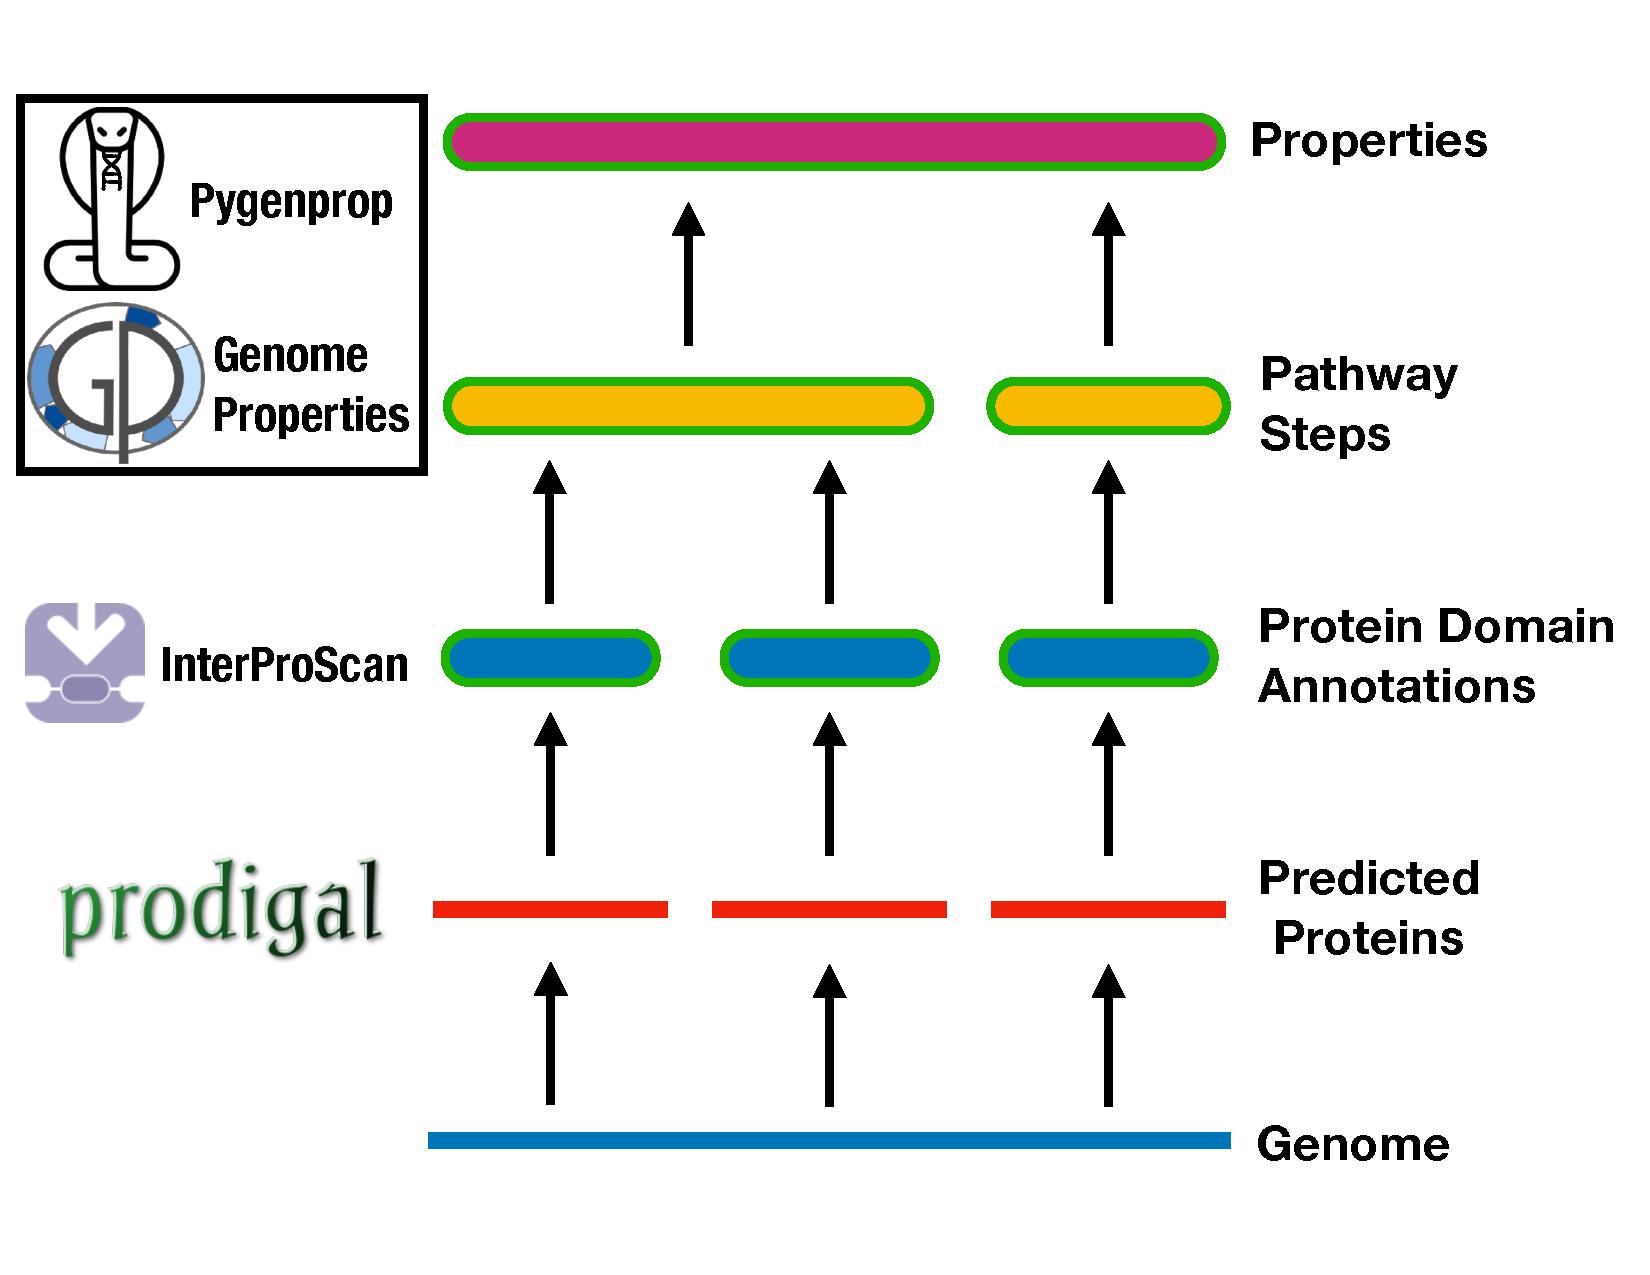
\includegraphics[width=0.8\textwidth]{media/micromeda-pipeline.pdf}
	 \caption[Steps performed and software tools used by Micromeda to predict the 
genome properties of an organism.]{\textbf{Steps performed and software tools 
used by Micromeda to predict the genome properties of an organism.} For 
prokaryotes, proteins must first be predicted via Prodigal. These proteins are 
then scanned using InterProScan5. The results of InterProScan are then combined 
with the Genome Properties database to predict pathways steps. These predictions 
are carried out by Pygenprop, which also predicts the overall presence and 
absence of pathways.}
	 \label{fig:micromeda-levels}
\end{figure}

\begin{figure}[!ht]
  \centering
	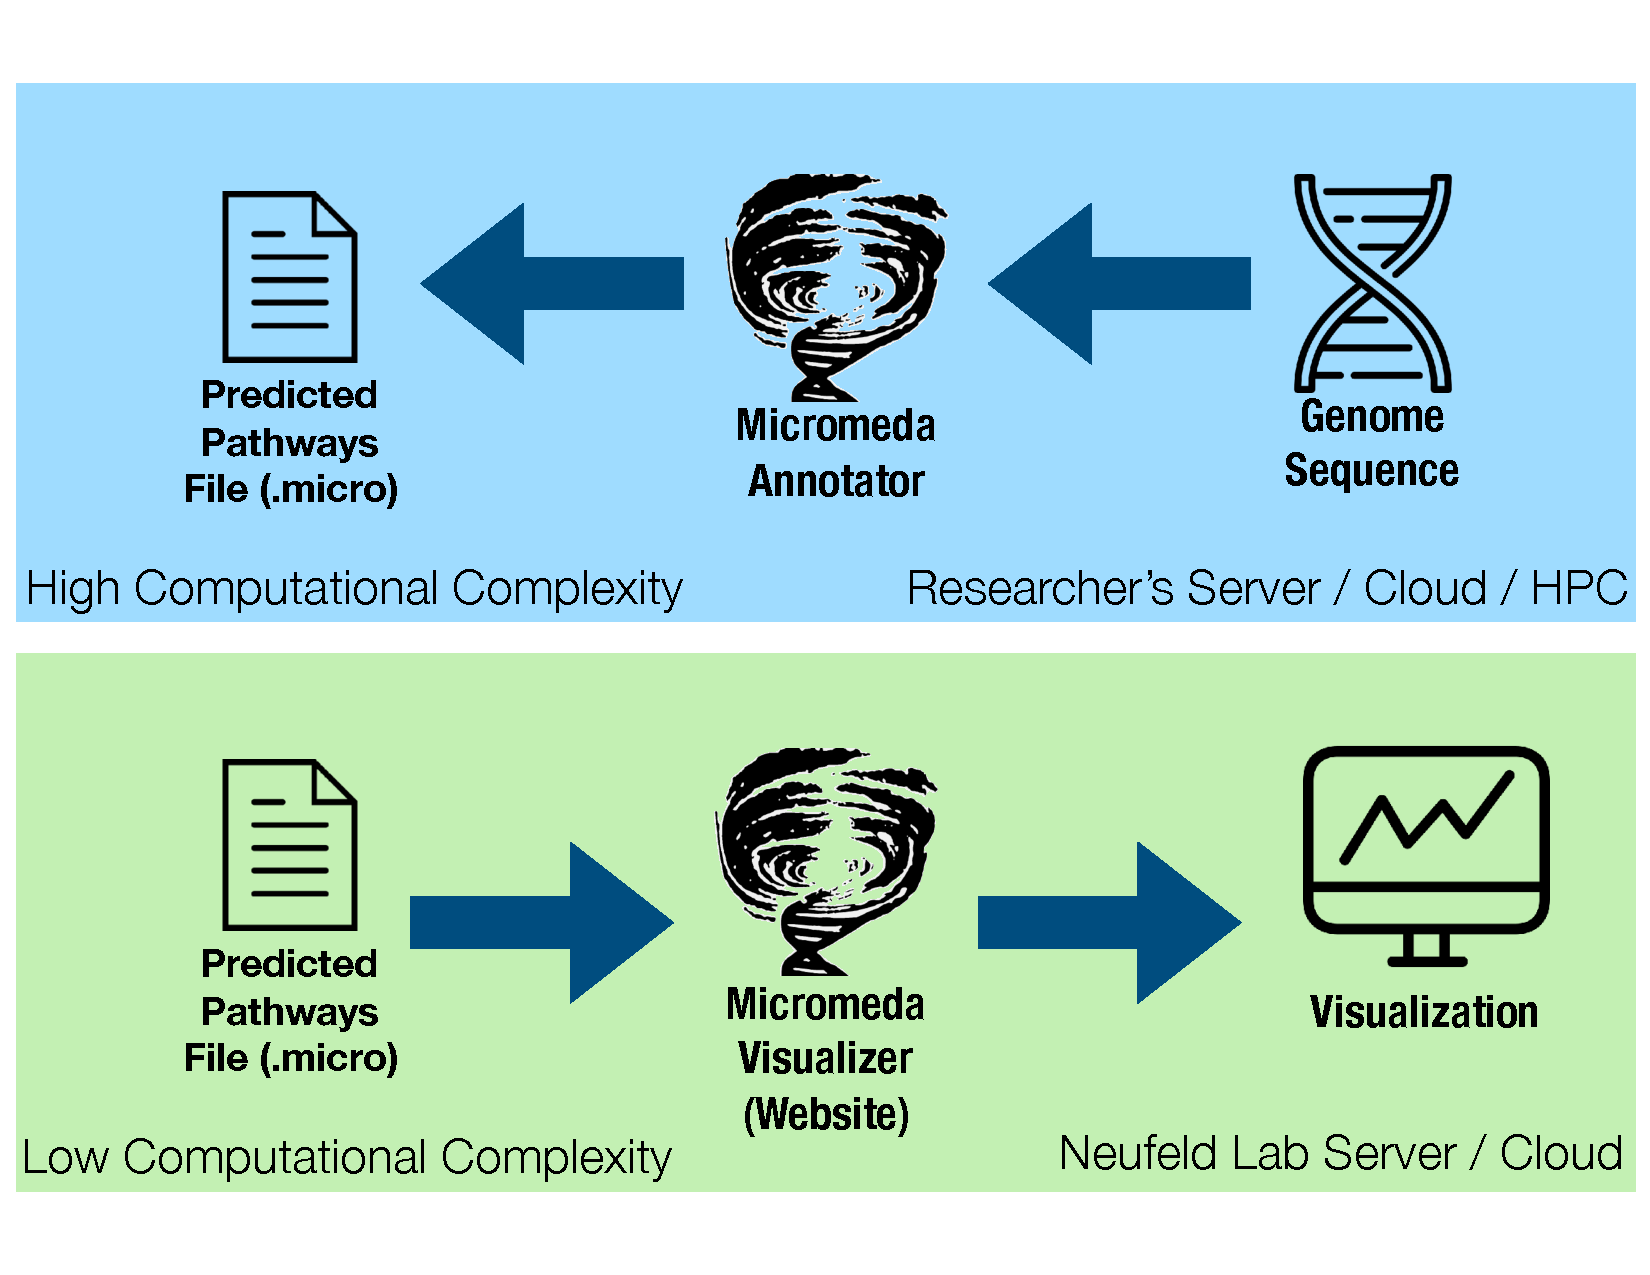
\includegraphics[width=0.8\textwidth]{media/micromeda-file-generation.pdf}
	 \caption[Two core steps that users must perform to generate Genome Properties 
visualizations using Micromeda.]{\textbf{Two core steps that users must perform 
to generate Genome Properties visualizations using Micromeda.} A local computer 
system must be used to execute a data generation step that creates a Micromeda 
file. Users can then upload this file to a second remote computer system that 
generates heat map visualizations. The most computationally complex step, 
Micromeda file generation, is not performed on the same server that generates 
the data visualizations.}
	 \label{fig:micromeda-file-generation}
\end{figure}

\begin{figure}[!ht]
  \centering
	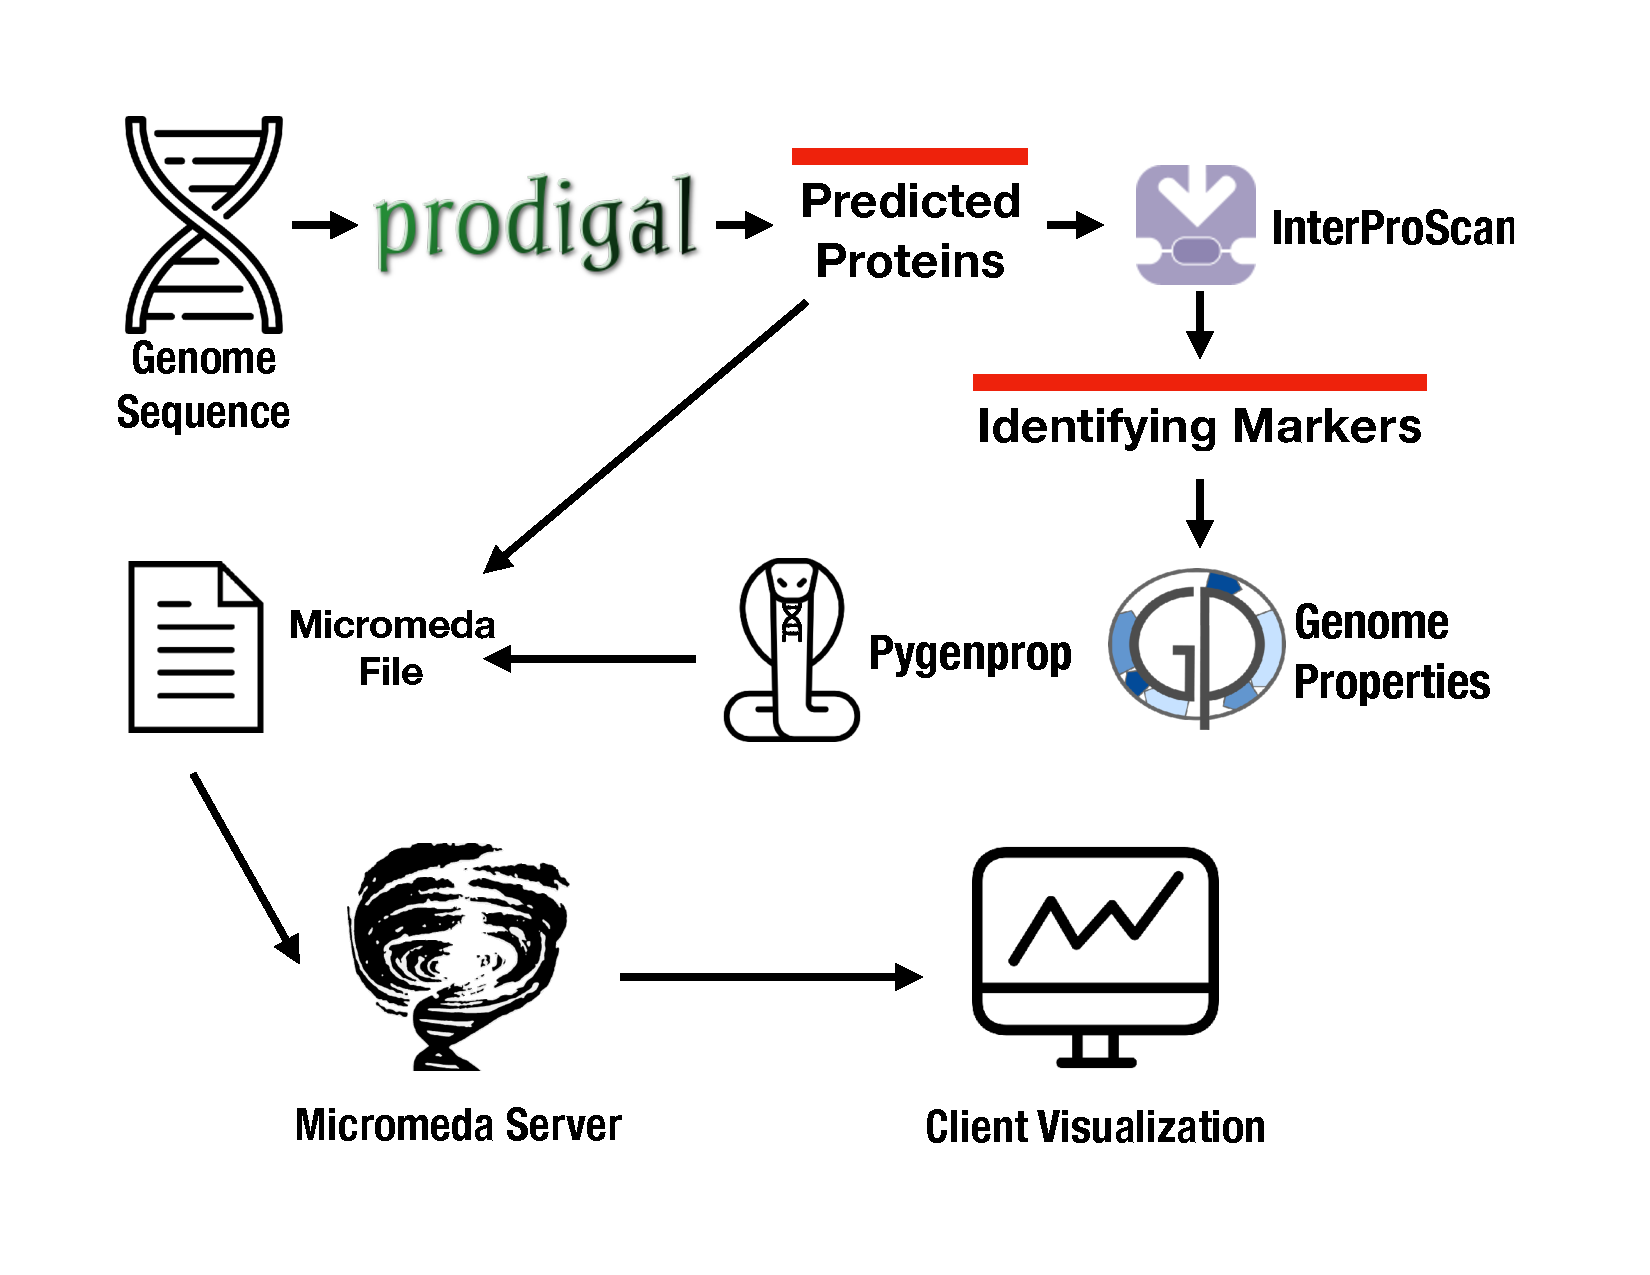
\includegraphics[width=0.8\textwidth]{media/how-micromeda-files-are-built.pdf}
	 \caption[How Micromeda files are built from InterProScan annotations of an 
organism's predicted proteins.]{\textbf{How Micromeda files are built from 
InterProScan annotations of an organism's predicted proteins.} These files 
possess not only pathway annotations but also the protein sequences that support 
these annotations. Thus, Micromeda files allow for the transfer of complete 
pathway analysis datasets. Such files can be uploaded to a remote server for visualization.}
	 \label{fig:micromeda-file-building-and-use}
\end{figure}

The Micromeda platform can be subdivided into two core components: a 
toolchain for generating Micromeda files (labelled Micromeda Annotator in Fig. 
\ref{fig:micromeda-file-generation}) and a web application for visualizing the 
data these files contain (labelled Micromeda Visualizer in Fig. 
\ref{fig:micromeda-file-generation}). The individual steps for generating 
Micromeda files can be done manually using only three \gls{cli} tools (see Fig. 
\ref{fig:micromeda-levels}, Fig. \ref{fig:micromeda-file-building-and-use}, and  
\href{http://en.wikipedia.org/wiki/Command-line_interface}{en.wikipedia.org/wiki/Command-line\_interface}). 
For example, with prokaryotic genomes, Prodigal could be used to predict protein 
sequences from an organism's genome sequence, and InterProScan5 could be used to 
scan these proteins to identify enzymes that support the existence of specific 
pathways (Fig. \ref{fig:micromeda-file-building-and-use}). Pygenprop contains a 
\gls{cli} (see 
\href{https://github.com/Micromeda/pygenprop#command-line-interface-cli}{github.com /Micromeda/pygenprop\#command\-line\-interface\-cli}) 
that is automatically installed when the library is installed on a user’s 
computer. This \gls{cli} allows users to generate Micromeda files from the 
output domain annotation \gls{tsv} files generated by InterProScan. A tutorial 
that covers how to generate Micromeda files can be found at 
\href{https://github.com/Micromeda/micromeda-workflow}{github.com/Micromeda/micromeda-workflow}.

\subsection{Micromeda Software Architecture Overview} \label{why-micromeda-files}

Micromeda follows a client-server web architecture \cite{svobodova1985client} 
(see 
\href{http://en.wikipedia.org/wiki/Client-server_model}{en.wikipedia.org/wiki/Client-server\_model} 
and Section \ref{web-servers}). Users interact with Micromeda-Client via their 
web browser, and this client allows them to upload Micromeda files to 
Micromeda-Server. Micromeda files contain all the information that the client 
requires to generate a pathway heat map. These files store pathway annotations, 
InterProScan5 output data, and supporting protein sequences for multiple 
organisms (see Section \ref{MicromedaFiles}). Having all these datasets in a 
single file simplifies the data upload process as only one file has to be 
uploaded by the user per heat map drawn. After upload, the contents of the 
uploaded file are stored temporarily in \gls{ram} on the computer used to host 
Micromeda-Server (see Section \ref{server-workflow}). Micromeda-Client will ask 
Micromeda-Server for data from this file as the client draws a heat map or 
responds to user activity (see Section \ref{client-implementation}). Multiple 
users can interact with Micromeda-Server and Client simultaneously\footnote{The 
number of simultaneous users that Micromeda-Server can support almost entirely 
depends on the server computer systems the software is run on and the deployment 
strategy used (see Subsection \ref{multi-server-micromeda-deployment}). 
Information about the scalability of Micromeda-Server, when running on a single 
computer, can be found toward the end of Section \ref{server-workflow}}.

Micromeda's \gls{ui} runs inside a user's web browser. The reasoning for using 
this approach, in contrast to building Micromeda as a native desktop 
application, is the approach's relative ease of deployment. End users only need 
to open the web address for the client to be loaded into their web browser and 
run. Because the application is web browser-based, it will work on any operating 
system with a modern web browser, including mobile devices such as tablet 
computers and cell phones.

Micromeda files exist is that they allow the rapid transfer of pathway 
annotation datasets that, in turn, allow for a separation of data generation and 
visualization. This separation is essential because there are vast computational 
complexity differences between generating pathway annotations and visualizing 
them. Micromeda's pathway prediction method involves identifying 
specific enzymes by running InterProScan5 on the set of all predicted proteins 
of an organism. The algorithms used by InterProScan5 are very computationally 
complex. It takes on the order of two hours to scan through the 4313 proteins of 
\textit{E. coli} K12 (\gls{ncbitaxa}: 1010810) using 100\% of all the \gls{cpu} 
cores of a 16 core server\footnote{InterProScan5 was tested on a server with two 
Intel E5310 (4 \gls{cpu} cores/4 threads/8 \gls{mb} cache/1.60 \gls{ghz} clock 
speed) processors and 16 \gls{gb}  of \gls{ram}.}.

In contrast, Micromeda can render a pathway heat map for over forty organisms in 
less than a second. Thus, if one wanted to have a web application that both 
computes and visualizes pathway annotations for uploaded genome sequences, then 
this application would require the support of an extensive and well-maintained 
hardware infrastructure. Developing the code to build, maintain, and sustain 
such a system draws away from the core goal of the Micromeda platform, which was 
to design a tool that helps users visualize pathway differences across 
organisms. Hence, for Micromeda, I chose to have users generate pathway 
annotations locally, using InterProScan5 and other tools, and have them upload 
these files to a remote web server for visualization (Fig. 
\ref{fig:micromeda-file-generation}). This design decision significantly reduces 
the hardware requirements for those who want to host Micromeda-Server and 
Client. The decision also reduces the overall design complexity of 
Micromeda-Client and Server and allows future development to focus on creating 
better and more feature-rich versions of Micromeda's \gls{ui} and 
visualizations.

\subsection{An Overview of the Data Sources Used by Micromeda: the Genome 
Properties Database, InterPro, and InterProScan5} \label{genome-properties} 

The architecture and implementation of Micromeda's components, such as Pygenprop 
and Micromeda-Client, are tied closely to the structure of the Genome Properties 
database. Thus, it is pertinent to discuss the database's structure. As 
mentioned in Section \ref{micromeda-overview}, Micromeda uses Pygenprop to 
predict the biochemical pathways possessed by an organism. These predictions are 
made by providing Pygenprop with a copy of the Genome Properties database and 
the output of running InterProScan5 on the organism's predicted proteins. In 
addition to discussing the structure of the Genome Properties database, this 
chapter will also discuss how domain annotations produced by InterProScan5 are 
combined with mappings from the Genome Properties database to generate pathway 
predictions.

\subsubsection{The InterPro Consortium of Protein Databases} \label{InterProDatabases}

Because the enzymes that carry out elements of metabolism in different organisms 
are highly similar and often evolutionarily related, it is useful to categorize 
proteins into groups that carry out a single function or share specific domains. 
Protein databases record the function of these groups of proteins and their 
domains and also store copies of these protein's sequences. In the past, many of 
these databases were maintained, operated, and funded independently. However, in 
the past two decades, many of the operators of these protein databases have 
banded together to form the InterPro consortium 
\cite{apweiler2000interpro,hunter2008interpro,Hunter2009}, which is headed by 
the \gls{ebi}\cite{cook2015european,finn2016interpro}. As of 2019, the InterPro 
consortium of protein databases manages fourteen member databases 
\cite{finn2016interpro,Hunter2009}. Examples of member databases include 
\gls{pfam} \cite{bateman2004pfam}, \gls{tigr} \cite{Haft2013}, \gls{panther} 
\cite{mi2005panther}, the \gls{cdd} \cite{marchler2014cdd}, \gls{hamap} 
\cite{lima2008hamap}, PRINTS \cite{attwood2000prints} and many others. Hosting 
of many of these member databases has been moved to \gls{ebi} maintained 
servers. In addition to the member databases, the consortium also provides the 
InterPro database \cite{hunter2008interpro,finn2016interpro}, which is a 
meta-database that allows for mapping between identical records for the same 
protein or domain groups across member databases. Each protein or domain 
catalogued is given a global InterPro identifier (\textit{e}.\textit{g}., 
IPRXXXX) that is mapped to multiple identifiers for the same protein or domain 
within member databases (\textit{e}.\textit{g}., PFXXXX or TFXXXX) 
\cite{hunter2008interpro,finn2016interpro}.

An import feature of protein databases is the ability to take the sequence of a 
novel protein (\textit{i}.\textit{e}., a protein that is not currently in the database) and 
predict the placement and function of the protein's domains, which is a process called 
domain annotation. The search algorithms used by member databases of the 
consortium compare novel proteins to computational models (\textit{i}.\textit{e}., a profile) that 
represents the sequence diversity (\textit{i}.\textit{e}., not all domains from different proteins 
and organisms have the same sequence) of each domain in the database. If the 
novel protein possesses a region of high similarity to a model, then it is 
likely that the novel protein possesses the domain that the model represents. 
Because the member databases of the InterPro consortium were developed 
independently, the methods they use for sequence search also vary (Fig. 
\ref{fig:interpro-databases}). The majority of these databases use HMMER (Fig. 
\ref{fig:interpro-databases}) \cite{eddy2011accelerated}, which compares the 
sequence of a novel protein to a \gls{hmm} \cite{de2007hidden}.

\begin{figure}[!ht]
  \centering
	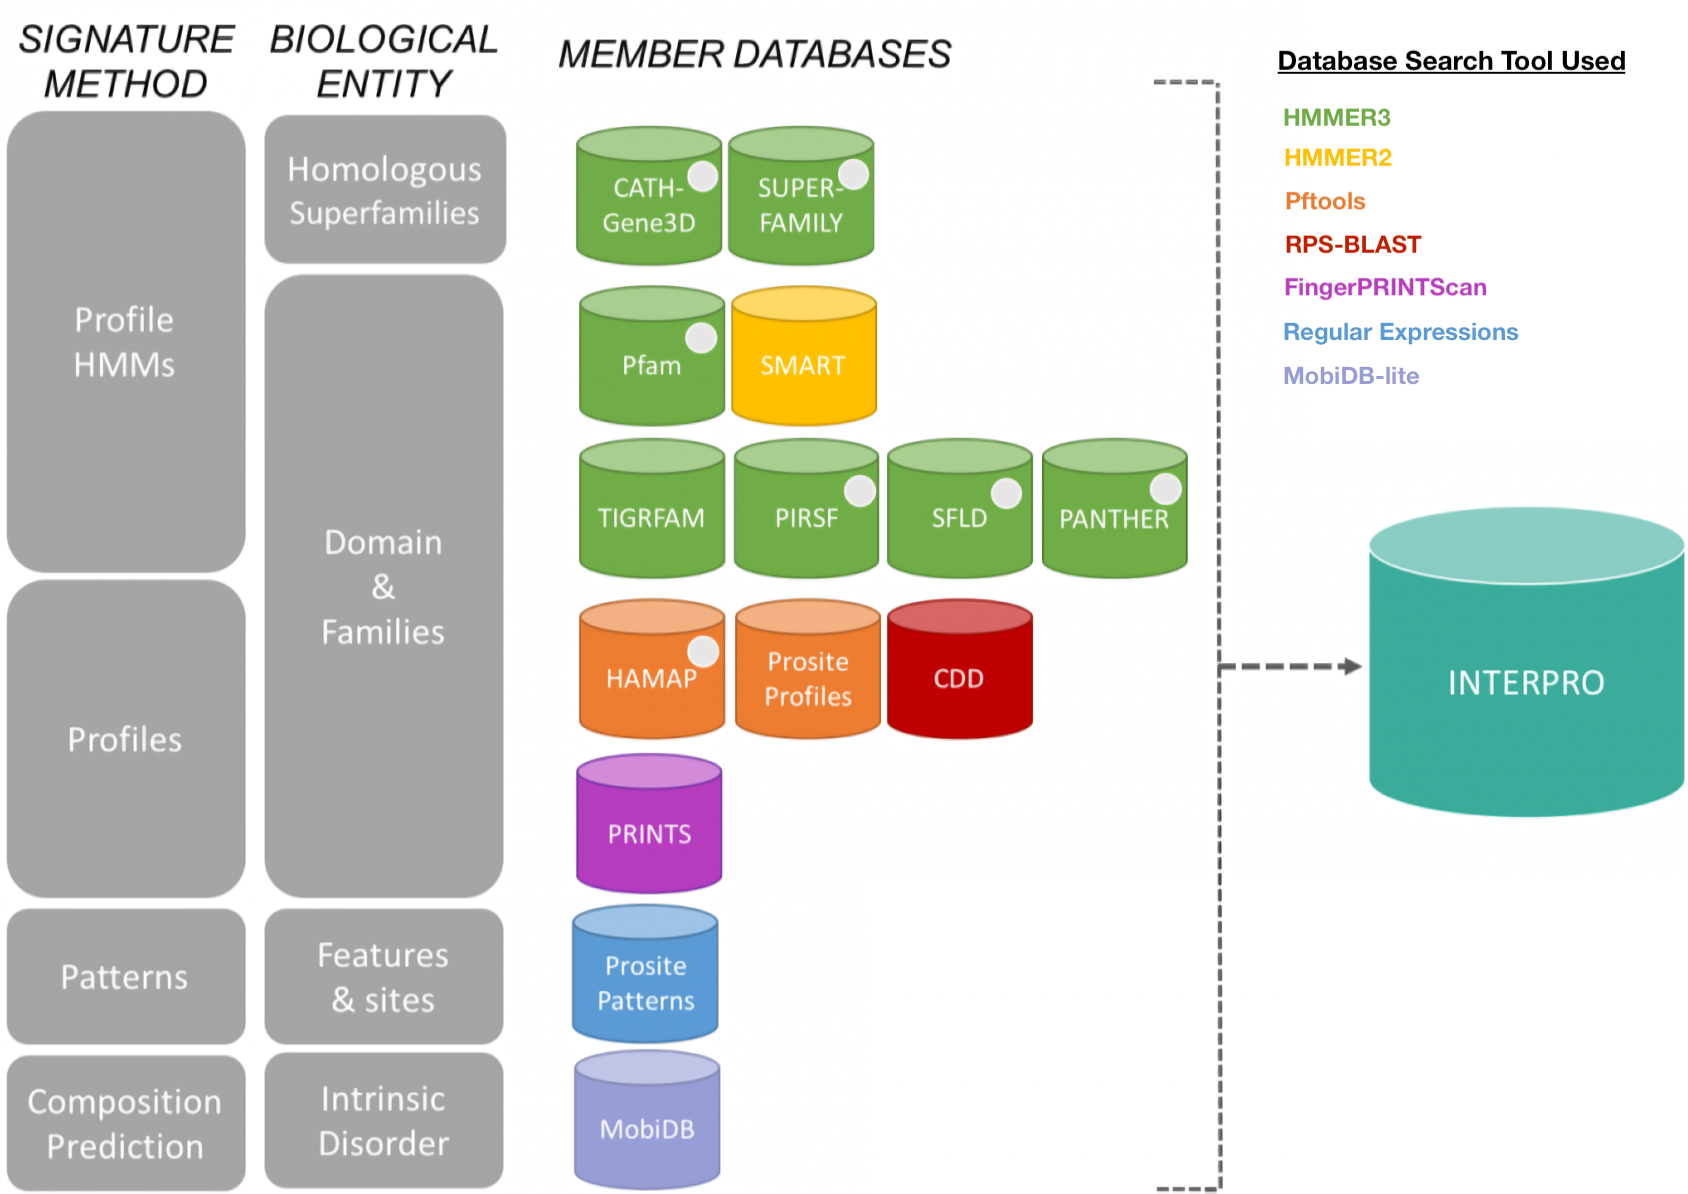
\includegraphics[width=\textwidth]{media/InterPro.png}
	 \caption[Member databases of the InterPro consortium and the model-based 
sequence search techniques that these databases use to classify novel protein 
sequences.]{\textbf{Member databases of the InterPro consortium and the 
model-based sequence search techniques that these databases use to classify 
novel protein sequences.} These search techniques require that the databases 
store models that represent multiple proteins or proteins domains. Examples of 
such models include \gls{hmm}s and \gls{pssm}. Examples of software that use 
such models are HMMER \cite{eddy2011accelerated} or \gls{rpsblast} 
\cite{mcginnis2004blast}. This figure is modified from the one found at 
\href{https://www.ebi.ac.uk/training/online/course/introduction-protein-classification-ebi/protein-classification-resources-ebi-interpro}{https://www.ebi.ac.uk/training/online/course/introduction-protein-classification-ebi/protein-classification-resources-ebi-interpro}.}
	 \label{fig:interpro-databases}
\end{figure}

If a portion of an organism's protein and a model are highly similar in 
sequence, they form a match. The quality of this match can be quantified by 
metrics such as the \gls{eval} score. This \gls{eval} score captures how likely 
it is that the match is real (\textit{i}.\textit{e}., the organism's protein contains the 
domain) given the chance of finding an equivalent match randomly in other 
proteins. Another metric for match quality is the length of the region of high 
sequence similarity, the alignment, shared between the protein and the database 
domain. If it is determined that a match is of high quality, the aligned region 
of the organism's protein can be assigned the same name and function as the 
domain in the database.  As discussed in Chapter \ref{Pygenprop}, Pygenprop can 
generate Micromeda files that store such match information.

Each member database has algorithms for filtering out false positive matches, 
which are those that occur between a model and a region of a protein that does 
not carry out the same function as the domain that the model represents. The 
member databases perform this filtering by implementing unique cut-off values, 
such as minimum \gls{eval} scores or alignment lengths, that can be used to 
filter out matches that may be spurious. The cut-off values can be made unique 
to each model. 

\subsubsection{InterProScan} \label{overview-interproscan}

InterPro consortium created a tool, InterProScan, that allows users to compare a 
novel protein sequence to all domain models found within InterPro member 
databases. The tool is a software wrapper for and execution engine of the 
model-based sequence search techniques (\textit{e}.\textit{g}., HMMER 
\cite{eddy2011accelerated}) used by all member databases of the InterPro 
consortium. InterProScan also implements the false positive filtering techniques 
developed for each member database. The latest version of the software, 
InterProScan5, follows a Master/Worker architecture (see 
\href{http://en.wikipedia.org/wiki/Master/slave_(technology)}{en.wikipedia.org/wiki/Master/slave\_(technology)}) 
where a master process schedules jobs for many worker processes. Depending on 
the number of \gls{cpu} cores of the computer running InterProScan5, tens to 
hundreds of models can be run against a novel protein simultaneously. Due to its 
architecture, InterProScan5 can also run jobs across a compute cluster. Due 
to this scalability, InterProScan is capable of domain annotating every protein 
of a microorganism in only a few hours, depending on the computer the software 
is run on and the organism's genome size. InterProScan takes a \gls{fasta} file 
\cite{pearson19905} containing an organism's predicted proteins as input and 
writes domain annotations and match data to \gls{tsv} files. The match data 
includes supporting information such as \gls{eval} scores for matches and 
predicted domain start and stop points on the organism's annotated protein.

\subsubsection{The Genome Properties Database} \label{genome-properties-overview}

The backbone of Micromeda is the Genome Properties database \cite{Haft2013}. 
The Genome Properties database takes advantage of the identifiability provided 
by protein domains to map from combinations of protein domains to enzymes that 
carry out pathway steps. \cite{richardson2018genome}. This mapping is in 
contrast to most other pathway databases, which map from whole proteins to 
biochemical pathways. If all the required domains for a pathway step are present 
in an organism's proteins, then the step is considered present. The domains used 
as markers by the Genome Properties database are those catalogued within the 
InterPro consortium of protein databases 
\cite{apweiler2000interpro,richardson2018genome}. 

The database goes beyond metabolism to include other organism capabilities such as 
cell motility (\textit{e}.\textit{g}., the presence of flagella and chemotaxis) 
and even microbial viral immunity mechanisms such a CRISPR/Cas9 
\cite{horvath2010crispr}. Within the database each capability is called a genome 
property. Multiple steps support each property, and each of these is supported 
by evidence that can be found from an organism's genome such as the presence of 
InterPro domains (\textit{e}.\textit{g}., \gls{pfam} \cite{bateman2004pfam}, 
\gls{tigr} \cite{haft2001tigrfams}, or \gls{cdd} \cite{marchler2014cdd} domains) 
in predicted proteins. Several genome properties are required as lines of 
evidence by others, and thus the database forms a rooted \gls{dag} (see 
\href{http://en.wikipedia.org/wiki/Directed_acyclic_graph}{en.wikipedia.org/wiki/Directed\_acyclic\_graph}) 
of connected properties. There are five types of genome properties: pathways, 
metapathways, systems, guilds, and categories (see 
\href{http://genome-properties.readthedocs.io/en/latest/flatfile.html#genome-property-types}{genome-properties.readthedocs.ioen/latest/flatfile.html\#genome-property-types} 
for details). The initial release of \gls{ebi} Genome Properties, version 1.0 
(January 9, 2018), had 584 properties and 3083 steps. The latest public release 
of the Genome Properties database, version 2.0 (August 30, 2018), contains 1296 
properties and 6525 steps \cite{richardson2018genome}. One of the core goals of 
the latest release was to expand the database beyond prokaryotic properties to 
include properties that are only possessed by eukaryotes or are shared between 
prokaryotes and eukaryotes. Version 2.0 has also incorporated pathways from 
MetaCyc \cite{karp2002metacyc}. The next version of the database, version 3.0, 
is still in active development and is planned to be released in spring 2020 (see 
\href{http://github.com/ebi-pf-team/genome-properties/issues/30#issuecomment-557090961}{github.com/ebi-pf-team/genome-properties/issues/30\#issuecomment-557090961}). 
Version 3.0 will contain fixes to existing properties, the addition of new 
properties\footnote{There is no ceiling to the number of properties that could 
be added to the Genome Properties database. As long as domains catalogued by the 
InterPro consortium can identify the proteins involved in a pathway or 
structure, then a property representing the pathway or structure can be 
generated.} and code fixes to the Genome Properties Perl library (see 
\href{http://github.com/ebi-pf-team/genome-properties/tree/rel3.0}{github.com/ebi-pf-team/genome-properties/tree/rel3.0}). 
Section \ref{genomeprop-oop} discusses how Pygenprop represents the structure of 
the Genome Properties database in memory.

If a specified number of required steps are found within the domain annotations 
of an organism's proteins, then the organism is understood to posses a specific 
genome property. The process of predicting what properties are possessed by an 
organism is called property assignment. To assign properties to an organism, 
InterProScan is first used to domain annotate all of its predicted proteins 
(\textit{e}.\textit{g}., those produced by Prodigal), and these annotations are then combined with 
information from the Genome Properties database to assess what properties are 
supported. Each property in the database is assigned YES, PARTIAL, and NO 
support. With Micromeda, Pygenprop is used to carry out these assessments. The 
Genome Properties database is provided to Pygenprop in the form of a release 
file, whose contents are detailed in the Subsection \ref{Genome-Properties-Files}. 
Subsection \ref{AssignmentCachingAlgorithm} details the exact algorithms used
for generating assignments.  

During the development of Micromeda, there were four reasons for selecting the 
Genome Properties database over other databases and InterProScan over other 
search tools. These reasons are explained below.

One of the primary reasons for using the Genome Properties database and 
InterProScan is that they allow pathway annotations to be built from domains 
identified by model-based search tools such as HMMER \cite{eddy2011accelerated} 
or \gls{rpsblast} \cite{mcginnis2004blast}. When compared to non-position
specific \gls{blast}-based \cite{altschul1990basic} search methods, which are 
commonly used by other pathway annotation systems, these model-based tools are 
better at detecting enzymes whose sequences are phylogenetically divergent from 
those previously known \cite{eddy2011accelerated}. This improved detection 
capability provides Micromeda with an advantage when it is applied to the 
genomes of previously unstudied organisms.

The Genome Properties database being domain-based also provides Micromeda with 
another advantage. Because the database is based on domains rather than whole 
proteins, Micromeda can detect the presence of enzymes that are split across 
multiple genes or have fused with other proteins. In a recent study that focused 
on confirming genome-predicted amino-acid auxotrophy across a variety of 
bacteria, the authors found that many predicted instances of auxotrophy were 
misannotations \cite{price2018filling}. Many of these misannotations were the 
result of either gene fusions or the enzyme being split across multiple genes 
\cite{price2018filling}. Traditional whole protein sequence-based detection 
methods such as \gls{blast} \cite{altschul1990basic}, which are typically used 
by pathway annotation pipelines based on databases such as \gls{kegg}, were 
shown to miss these enzymes \cite{price2018filling}. For example, if previous 
forms of a protein were all found to be encoded by a single gene, such whole 
sequence methods were shown to filter out versions of the enzyme that are split 
across genes due to inadequate alignment lengths for matches to individual 
subunits \cite{price2018filling}. In contrast, InterProScan will detect all 
required domains, whether the proteins are on one gene or multiple.

Another advantage of Genome Properties is that it is freely available under an 
open-source licence and hosted on GitHub \cite{richardson2018genome}. In 
contrast, two of the most prominent pathway databases, \gls{kegg} and BioCyc 
\cite{karp2005expansion}, have been commercialized. \gls{kegg}'s website is free 
for academic use in terms of using the data held within for hypothesis testing 
(see \href{http://www.kegg.jp/kegg/legal.html}{kegg.jp/kegg/legal.html}). 
However, bulk download of the entire database, as would be required for a 
pathway annotation system such as Micromeda, has a licensing fee of \$2000 
\gls{usd} per year (as of 2019 and see 
\href{https://www.bioinformatics.jp/docs/subscription_fees.pdf}{bioinformatics.jp/docs/subscription\_fees.pdf}). 
This fee increases to \$5000 \gls{usd} per year if a user ``provide[s] any 
outside service using... \gls{kegg} data" (as of 2019 and see 
\href{https://www.bioinformatics.jp/docs/subscription_fees.pdf}{bioinformatics.jp/docs/subscription\_fees.pdf}). 
Thus, if Micromeda were built around the \gls{kegg} database, users creating 
Micromeda files would be required to pay \$2000 \gls{usd} per year, and any user 
hosting Micromeda server, as a public service, would be required to pay \$5000 
\gls{usd} per year. BioCyc follows a similar paid scheme 
(\href{http://metacyc.org/download.shtml}{metacyc.org/download.shtml}). 

The Genome Properties database has also been shown to have comparable coverage, 
in terms of organism proteins used to support the existence of pathways, to 
databases such a \gls{kegg} and Seed Subsystems \cite{richardson2018genome}. 
This coverage was consistent across a variety of microbes from distant taxonomic 
clades \cite{richardson2018genome}. Thus, there is no high-level database 
completeness disadvantage if Micromeda uses the Genome Properties database. 

\section{Summary} \label{introduction_summary}

When Micromeda performs pathway annotation, it does so based on the presence of 
InterPro domains found within organisms' predicted proteomes. These domains are 
detected using model-based sequence search software that is orchestrated by 
InterProScan5. The contents of the Genome Properties database is used to map 
from the presence of domains to the presence of genome property steps. The 
presence of steps is used to infer YES, PARTIAL, or NO support for individual 
genome properties. The model-based search techniques used by InterProScan allow 
Micromeda to provide highly accurate and comprehensive results with no licensing 
fees.

Micromeda allows users to visualize the differences in pathway presence and 
absence across organisms. The tool generates visualizations based on the data 
contained within uploaded Micromeda files. Pygenprop is a software library that 
can not only produce Micromeda files but also make programmatic comparisons of 
pathway presence and absence across organisms. Potential improvements to 
individual components of Micromeda are highlighted in the summary section of 
each of their chapters. Potential improvements that would require modification 
of multiple components are highlighted in Chapter \ref{conclusion-chapter}. As 
discussed in Chapter \ref{conclusion-chapter}, Micromeda breaks new ground in 
both features and implementation and will increase both the speed and ease at 
which researchers perform pathway analysis.
